\documentclass[11pt]{article}
\usepackage{tikz}
\usetikzlibrary{shapes, arrows}
\usepackage[hmargin=1in,vmargin=1in]{geometry}
\usepackage{xcolor}
\usepackage{enumitem} 
\usepackage{wrapfig}
\usepackage{amsmath,amssymb,amsfonts,url,sectsty,framed,tcolorbox,framed}
\newcommand{\pf}{{\bf Proof: }}
\newtheorem{theorem}{Theorem}
\newtheorem{lemma}{Lemma}
\newtheorem{proposition}{Proposition}
\newtheorem{definition}{Definition}  
\newtheorem{remark}{Remark}
\newcommand{\qed}{\hfill \rule{2mm}{2mm}}
\usepackage{fixltx2e}
\usepackage{graphicx}
\begin{document}
	\noindent
	\rule{\textwidth}{1pt}
	\begin{center}
		{\bf [CS304] Introduction to Cryptography and Network Security}
	\end{center}
	Course Instructor: Dr. Dibyendu Roy \hfill Winter 2022-2023\\
	Scribed by : Pallikonda Sai Teja  \hfill Lecture (Week 03)\\
	Student ID:202011052\\
	\\
	\rule{\textwidth}{1pt}
	\section{One Time Padding OTP}
	\flushleft $\rightarrow$ OTP provides perfect secrecy under some conditions.\\
	\centering Pr[message $|$ ciphertext] = Pr[message]
	\flushleft
	\section{OTP on one bit encryption}
	m $\in$ \{0,1\} $\Rightarrow$ Message \hspace{2cm} K $\in$ \{0,1\} $\Rightarrow$ Key\\
	Pr[m=0] = p \hspace{3.5cm} Pr[k=0] = $1/2$ \\
	Pr[m=1] = 1-p \hspace{3.2cm} Pr[k=1] = $1/2$\\
	
	\subsection{Encryption}
	c = m $\oplus$ k \\
	c = 0 $\Rightarrow$ \{m = 0,k = 0\} $\displaystyle \cup$ \{m = 1,k = 1\}\\
	Pr[c = 0] = Pr[m = 0,k = 0] + Pr[m = 1,k = 1]\\
	\hspace{1.7cm}= p * $1/2$ + (1 - p) * $1/2$ \\
	\hspace{1.7cm}= $p + 1 - p/2$\\
	\hspace{1.7cm}= $1/2$
	
	Pr[c = 1] = 1 - Pr[c = 0]\\
	\hspace{1.7cm}= 1 - $1/2$\\
	\hspace{1.7cm}= $1/2$
	
	Pr[M = m $/$C = c] =? Pr[M = m]\\
	Pr[M = 0 $/$C = 0] = $\frac{Pr[M = 0\hspace{0.1cm} \cap\hspace{0.1cm}\ C = 0]}{Pr[C = 0]}$ \hfill Pr[$A/B$] = Pr[A $\displaystyle \cap$ B]/Pr[B]\\
	\hspace{3.4cm}= $\frac{Pr[C = 0/M = 0] * Pr[M = 0]}{1/2}$ \hfill Pr[A $\displaystyle \cap$ B] = Pr[$B/A$] * Pr[A] \\
	\hspace{3.4cm}= $\frac{1/2 \hspace{0.1cm}*\hspace{0.1cm} Pr[M = 0]}{1/2}$\\
	\hspace{3.4cm}= Pr[M = 0]\\
	Pr[M = 0 $/$C = 0] = Pr[M = 0]\\
	\centering{Thus it provides perfect secrecy}\\
	\flushleft
	\subsection*{Conditions}
	\begin{enumerate}
		\item M\textsubscript1 $\oplus$ k = c\textsubscript1 \\
		M\textsubscript2 $\oplus$ k = c\textsubscript2 \hspace{1cm} This will reveal information of messages\\
		c\textsubscript1 $\oplus$ c\textsubscript2 = (M\textsubscript1 $\oplus$ k) $\oplus$ (M\textsubscript2 $\oplus$ k)\\\hspace{1.4cm}= c\textsubscript1 $\oplus$ c\textsubscript2 = M\textsubscript1 $\oplus$ M\textsubscript2\\
		Hence cipher text difference will give us message difference
		\item Len(k) $<$ Len(P)\\
		c = P $\oplus$ k\\
		Example :\\
		32-bit message P\\
		16-bit key K\\
		P $\oplus$ k = P $\oplus$ 0...0K \hspace{1cm} 16-0bits are added to K\\
		Here first 16-bits of P are same as first 16-bits of ciphertext c \\
		\item Some part of key is repeated \\
		P = P\textsubscript{1}..P\textsubscript{l}..P\textsubscript{n} \hfill P\textsubscript{i} is bit at $i^{th}$ position\\ \vspace{.3cm}
		\hspace{0.33cm}P = P\textsubscript{1}...P\textsubscript{l}....P\textsubscript{n}\\
		$\oplus$ k = k\textsubscript{1}...k\textsubscript{l}k\textsubscript{1}..k\textsubscript{n}\\
		\begin{tikzpicture}
			\draw (0.33,0) -- (3.6,0);
		\end{tikzpicture}\\
		c = (P\textsubscript{1} $\oplus$ k\textsubscript{1})(P\textsubscript{2} $\oplus$ k\textsubscript{2})..(P\textsubscript{l} $\oplus$ k\textsubscript{l})(P\textsubscript{l+1} $\oplus$ k\textsubscript{1})..(P\textsubscript{n} $\oplus$ k\textsubscript{t})\\
		c\textsubscript{1} = (P\textsubscript{1} $\oplus$ k\textsubscript{1})\\
		c\textsubscript{l+1} = (P\textsubscript{l+1} $\oplus$ k\textsubscript{1})\\
		c\textsubscript{1} $\oplus$ c\textsubscript{l+1} = (P\textsubscript{1} $\oplus$ k\textsubscript{1}) $\oplus$ (P\textsubscript{l+1} $\oplus$ k\textsubscript{1})\\
		= P\textsubscript{1} $\oplus$ P\textsubscript{l+1}\\
		Information of the message is revealed.\\
	\end{enumerate}
	\mbox{*} OTP is not used in real life.
	\section{Data Encryption Standard (DES)}
	$\rightarrow$ It is a block cipher\\
	$\rightarrow$ It is designed by IBM\\
	\begin{enumerate}
		\item Block size = 64 bit
		\item Number of rounds = 16
		\item Secret key size = 64 bit including 8 parity check bits
		\item It is based on Feistel Network
	\end{enumerate}
	\subsection{Encryption}
	\centering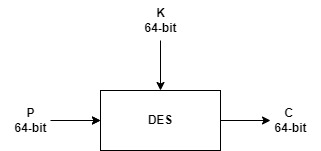
\includegraphics[width = 8cm]{Encryption.jpg}
	\flushleft
	\subsection{Decryption}
	\centering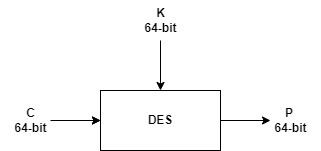
\includegraphics[width = 8cm]{Decryption.jpg}
	\flushleft
	\mbox{*} Secret key is 64 bit with 8 parity check bits.\\
	$8^{th}$,$16^{th}$,....,$64^{th}$ bits are parity check bits.\\
	\mbox{*} In DES, we have 16 round keys k\textsubscript{1},k\textsubscript{2},..,k\textsubscript{16}\\
	Which are generated using Key scheduling algorithm. Key scheduling algorithm will take the secret key as an input.\\
	len(k\textsubscript{i}) = 48 bit.\hfill G(k) $\rightarrow$ k\textsubscript{1},k\textsubscript{2},..,k\textsubscript{16}
	\section{Structure of DES}
	\centering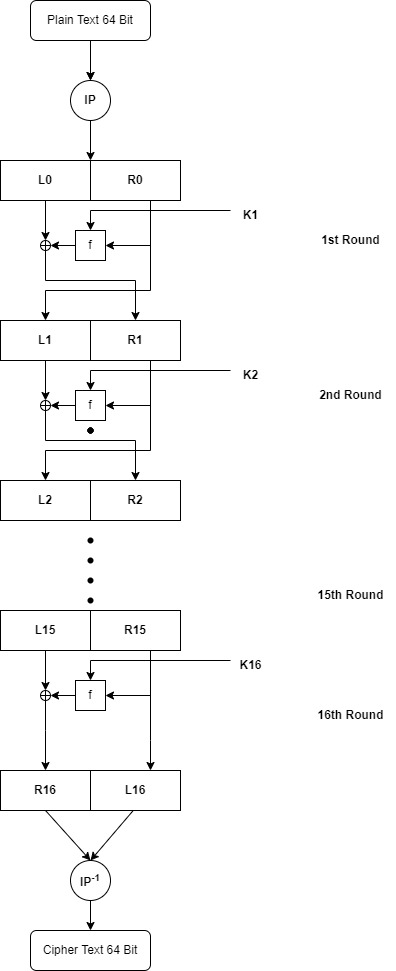
\includegraphics[width = 5.2cm]{DES.jpg}
	\flushleft\subsection{Encryption}
	$$f : \{0,1\}^{32} x \{0,1\}^{48} \rightarrow \{0,1\}^{32}$$\\
	L\textsubscript{i+1} = R\textsubscript{i}\\
	R\textsubscript{i+1} = L\textsubscript{i} $\oplus$ f(R\textsubscript{i},k\textsubscript{i+1})\\
	\subsection*{We have to learn the following}
	\begin{itemize}
		\item $IP, IP^{-1}$.
		\item What is f (Round function).
		\item How k\textsubscript{1},k\textsubscript{2},..,k\textsubscript{16} are generated?
	\end{itemize}
	\subsection{IP (Initial Permutation)}
	$$IP : \{0,1\}^{64} \rightarrow \{0,1\}^{64}$$
	IP :
	\begin{tabular}{ c c c c c c c c }
		58 & 50 & 42 & 34 & 26 & 18 & 10 & 2\\ 
		60 & 52 & 44 & 36 & 28 & 20 & 12 & 4\\  
		62 & 54 & 46 & 38 & 30 & 22 & 14 & 6\\
		64 & 56 & 48 & 40 & 32 & 24 & 16 & 8\\
		57 & 49 & 41 & 33 & 25 & 17 & 9 & 1\\
		59 & 51 & 43 & 35 & 27 & 19 & 11 & 3\\
		61 & 53 & 45 & 37 & 29 & 21 & 13 & 5\\
		63 & 55 & 47 & 39 & 31 & 23 & 15 & 7
	\end{tabular}\\
	IP(m\textsubscript{1},m\textsubscript{2},..,m\textsubscript{64}) = (m\textsubscript{58},m\textsubscript{50},m\textsubscript{42},m\textsubscript{34},..,m\textsubscript{7})\\
	\subsection{$IP^{-1}$ (Final Permutation)}
	$$IP : \{0,1\}^{64} \rightarrow \{0,1\}^{64}$$
	IP :
	\begin{tabular}{ c c c c c c c c }
		40 & 8 & 48 & 16 & 56 & 24 & 64 & 32\\ 
		39 & 7 & 47 & 15 & 55 & 23 & 63 & 31\\  
		38 & 6 & 46 & 14 & 54 & 22 & 62 & 30\\
		37 & 5 & 45 & 13 & 53 & 21 & 61 & 29\\
		36 & 4 & 44 & 12 & 52 & 20 & 60 & 28\\
		35 & 3 & 43 & 11 & 51 & 19 & 59 & 27\\
		34 & 2 & 42 & 10 & 50 & 18 & 58 & 26\\
		33 & 1 & 41 & 9 & 49 & 17 & 57 & 25
	\end{tabular}\\
	IP(m\textsubscript{1},m\textsubscript{2},..,m\textsubscript{64}) = (m\textsubscript{40},m\textsubscript{8},m\textsubscript{48},m\textsubscript{16},..,m\textsubscript{25})\\
	\subsection{Round Function of DES}
	\centering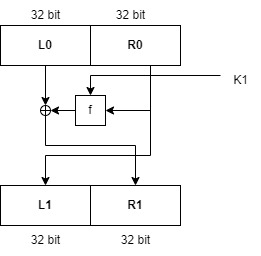
\includegraphics[width = 8.4cm]{Round Function of DES.jpg}
	\flushleft$$f : \{0,1\}^{32} x \{0,1\}^{48} \rightarrow \{0,1\}^{32}$$\\
	f(R\textsubscript{i},k\textsubscript{i}) = X\textsubscript{i}\\
	where,\\
	R\textsubscript{i} is 32 bit\\
	k\textsubscript{i} is 48 bit\\
	X\textsubscript{i} is 32 bit\\
	$$f(R\textsubscript{i},k\textsubscript{i}) = P(S(E(R\textsubscript{i}) \oplus k\textsubscript{i}))$$\\
	$E : \{0,1\}^{32} \rightarrow \{0,1\}^{48}$ (Expansion Function)\\
	$S : \{0,1\}^{48} \rightarrow \{0,1\}^{32}$ (Substitution Box)\\
	$P : \{0,1\}^{32} \rightarrow \{0,1\}^{32}$ (Permutation Box)\\
	\subsection{Expansion Function E}
	E :
	\begin{tabular}{ c c c c c c c c }
		32 & 1 & 2 & 3 & 4 & 5 \\ 
		4 & 5 & 6 & 7 & 8 & 9 \\  
		8 & 9 & 10 & 11 & 12 & 13 \\
		12 & 13 & 14 & 15 & 16 & 17 \\
		16 & 17 & 18 & 19 & 20 & 21 \\
		20 & 21 & 22 & 23 & 24 & 25 \\
		24 & 25 & 26 & 27 & 28 & 29 \\
		28 & 29 & 30 & 31 & 32 & 1 
	\end{tabular}\\
	E(x\textsubscript{1},x\textsubscript{2},..,x\textsubscript{32}) = (x\textsubscript{32},x\textsubscript{1},x\textsubscript{2},x\textsubscript{3},..,x\textsubscript{1})\\
	\subsection{Substitution S} 
	$S : \{0,1\}^{48} \rightarrow \{0,1\}^{32}$ \\
	
	\mbox{*} X = B\textsubscript{1}B\textsubscript{2}B\textsubscript{3}B\textsubscript{4}B\textsubscript{5}B\textsubscript{6}B\textsubscript{7}B\textsubscript{8}\\
	where length od B\textsubscript{i} is 6-bit.\\
	\mbox{*} S\textsubscript{1},S\textsubscript{2},S\textsubscript{3},S\textsubscript{4},S\textsubscript{5},S\textsubscript{6},S\textsubscript{7},S\textsubscript{8}\\
	$S\textsubscript{i} : \{0,1\}^{6} \rightarrow \{0,1\}^{4}$  $\forall$ i = 1,2,3,4,5,6,7,8\\
	S\textsubscript{i}(B\textsubscript{i}) = C\textsubscript{i}\\
	S(X) = (S\textsubscript{1}(B\textsubscript{1}),S\textsubscript{2}(B\textsubscript{2}),S\textsubscript{3}(B\textsubscript{3}),S\textsubscript{4}(B\textsubscript{4}),S\textsubscript{5}(B\textsubscript{5}),S\textsubscript{6}(B\textsubscript{6}),S\textsubscript{7}(B\textsubscript{7}),S\textsubscript{8}(B\textsubscript{8}))\\
	\mbox{*} B\textsubscript{i} = b\textsubscript{1}b\textsubscript{2}b\textsubscript{3}b\textsubscript{4}b\textsubscript{5}b\textsubscript{6} \hfill b\textsubscript{i} $\in$ \{0,1\}\\ 
	\mbox{*} r = (2*b\textsubscript{1} + b\textsubscript{6}) \hfill $0 \leq r \leq 3$\\
	\mbox{*} r is the representation of(b\textsubscript{1}b\textsubscript{6})\\
	\mbox{*} c is the representation of(b\textsubscript{2}b\textsubscript{3}b\textsubscript{4}b\textsubscript{5})\hfill $0 \leq c \leq 15$\\
	r $\rightarrow$ row number\\
	c $\rightarrow$ column number\\
	S\textsubscript{i}(B\textsubscript{i}) = a\textsubscript{r,c} $\rightarrow$ 4 bit
	\subsection{Permutation P} 
	$$P : \{0,1\}^{32} \rightarrow \{0,1\}^{32}$$\\
	P :
	\begin{tabular}{ c c c c }
		16 & 7 & 20 & 21 \\ 
		29 & 12 & 28 & 17 \\  
		1 & 15 & 23 & 26 \\
		5 & 18 & 31 & 10 \\
		2 & 8 & 24 & 14 \\
		32 & 27 & 3 & 9 \\
		19 & 13 & 30 & 6 \\
		22 & 11 & 4 & 25
	\end{tabular}\\
	P(x\textsubscript{1},x\textsubscript{2},..,x\textsubscript{32}) = (x\textsubscript{16},x\textsubscript{7},x\textsubscript{20},x\textsubscript{21},..,x\textsubscript{25})\\
	\subsection{We have to understand the key scheduling Algorithm.} 
	\begin{itemize}
		\item Input : 64 bit key K.
		\item Output : 16 round key k\textsubscript{i},1 $\leq$ i $\leq$ 16
	\end{itemize}
	len(k\textsubscript{i}) = 48 bit.
	\begin{enumerate}
		\item v\textsubscript{i}, 1 $\leq i \leq$ 16 where v\textsubscript{i} = 1\\
		if i $\in$ \{1,2,9,16\} else v\textsubscript{i} = 2.
		\item Delete the parity check bits. Now key k is 56 bits.
		\item T = PC1(k); $PC1 : \{0,1\}^{56} \rightarrow \{0,1\}^{56}$ 
		\item (C\textsubscript{0},D\textsubscript{0}) = T where C\textsubscript{0} is of 28 bit,D\textsubscript{0} is of 28 bit
		\item for i = 1 to 16\\
		C\textsubscript{i} = (c\textsubscript{i-1} left circular shift v\textsubscript{i})\\
		D\textsubscript{i} = (D\textsubscript{i-1} left circular shift v\textsubscript{i})\\
		k\textsubscript{i} = PC2(C\textsubscript{i},D\textsubscript{i}) \\
		PC2 : $\{0,1\}^{56} \rightarrow \{0,1\}^{56}$
		\item Round Keys = \{k\textsubscript{1},k\textsubscript{2},..,k\textsubscript{16}\}
	\end{enumerate}
	
	\textbf{PC1 : $\{0,1\}^{56} \rightarrow \{0,1\}^{56}$}\\
	c\textsubscript{i} :
	\begin{tabular}{ c c c c c c c }
		57 & 49 & 41 & 33 & 25 & 17 & 9 \\ 
		1 & 58 & 50 & 42 & 34 & 26 & 18\\  
		10 & 2 & 59 & 51 & 43 & 35 & 27\\
		19 & 11 & 3 & 60 & 52 & 44 & 36
	\end{tabular}\\
	d\textsubscript{i} :
	\begin{tabular}{ c c c c c c c }
		63 & 55 & 47 & 39 & 31 & 23 & 15\\ 
		7 & 62 & 54 & 46 & 38 & 30 & 22\\  
		14 & 6 & 61 & 53 & 45 & 37 & 29\\
		21 & 13 & 5 & 28 & 20 & 12 & 4
	\end{tabular}\\
	PC1(k\textsubscript{1},k\textsubscript{2},..,k\textsubscript{63}) = (k\textsubscript{57},x\textsubscript{44},x\textsubscript{41},x\textsubscript{33},..,x\textsubscript{4})\\
	
	PC2\textsubscript{i} :
	\begin{tabular}{ c c c c c c }
		14 & 17 &11& 24& 1 &5\\
		3 &28 &15& 6& 21 &10\\
		23 &19 &12& 4 &26& 8\\
		16 &7 &27 &20 &13& 2\\
		41 &52 &31 &37 &47 &55\\
		30 &40 &51 &45& 33 &48\\
		44 &49& 39& 56 &34& 53\\
		46 &42 &50 &36 &29 &32
	\end{tabular}\\
	
	\centering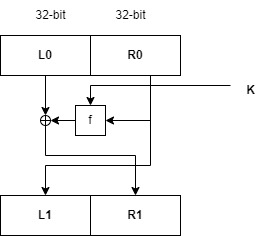
\includegraphics[width = 8.4cm]{DES 2 (1).jpg}
	\flushleft$$f(R\textsubscript{i},k\textsubscript{i}) = P(S(E(R\textsubscript{i}) \oplus k\textsubscript{i}))$$\\
	M = L\textsubscript{0}$\|$R\textsubscript{0}\\
	c\textsubscript{1} = L\textsubscript{1}$\|$R\textsubscript{1}\\
	FN(M,K) = c\textsubscript{1}\\
	FN($M^{c},K^{c}$) = c\textsubscript{2}\\ \hfill $X^{c}$ = bitwise complement of X\\
	L\textsubscript{1} = R\textsubscript{0}\\
	R\textsubscript{1} = L\textsubscript{0} $\oplus$ f(R\textsubscript{0},k)\\
	$k^c \oplus E(R^c)$ = $(E(R))^c \oplus k^c$ = E(R) $\oplus$ k\\
	P(S($k^c \oplus E(R^c)$)) = P(S(E(R) $\oplus$ k))\\
	L\textsubscript{0}$\|$R\textsubscript{0} = M \hspace{1cm} $L\textsubscript{0}^c\|R\textsubscript{0}^c = M^c$\\
	L\textsubscript{1} = R\textsubscript{0}\\
	R\textsubscript{1} = L\textsubscript{0} $\oplus$ f(R\textsubscript{0},k)\\
	$L\textsubscript{1}^c = R\textsubscript{0}^c$\\
	$R\textsubscript{1}^c = L\textsubscript{0}^c \oplus f(R\textsubscript{0}^c,k^c) = L\textsubscript{0}^c \oplus f(R\textsubscript{0},k)$ = $(L\textsubscript{0} \oplus f(R\textsubscript{0},k))^c = R\textsubscript{1}^c$\\
	c\textsubscript{1} = L\textsubscript{1}$\|$ R\textsubscript{1}\\
	$c\textsubscript{2} = L\textsubscript{1}^c\| R\textsubscript{1}^c$\\
	$$c\textsubscript{2} = c\textsubscript{1}^c$$
\end{document}
